\documentclass{ximera}

\title{Rates of Change in Applications Activity}
\author{MATH 425: Calculus I}

\begin{document}
\begin{abstract}
    Working with the peers in your group, solve the following problems. Make sure to show and justify all your work. Make sure everyone in the group understands the solution and participates. Be prepared to report your answers to the whole class. 
\end{abstract}
\maketitle


\begin{exercise}
    The following graph shows the height $y$ of a mass oscillating at the end of a spring, through one cycle of oscillation.  Sketch the graph of the velocity as a function of time from the graph.
    \begin{image}
        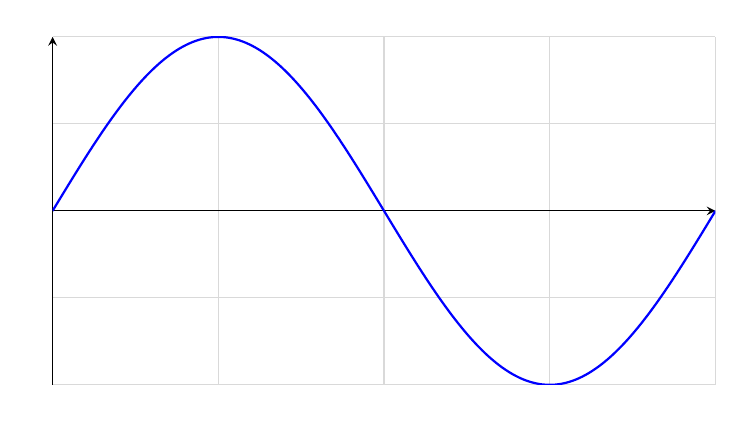
\begin{tikzpicture}
            \begin{axis}[
                width=10cm,
                height=6cm,
                grid=major,
                grid style={gray!30},
                xtick={0, 1.5708, 3.1416, 4.7124, 6.2832},
                xtick style={draw=none},
                ytick style={draw=none},
                xticklabels={},
                yticklabels={},
                axis lines=middle,
            ]
                \addplot[blue, thick, domain=0:2*pi, samples=200] {sin(deg(x))};
            \end{axis}
        \end{tikzpicture}
    \end{image}
    %\xmalt Graph of one period of a $\sin(x)$-looking curve.
\end{exercise}

\begin{exercise}
    Suppose that for $x\geq 1000$, the dollar cost of producing $x$ video cameras is $$C(x)=500x-0.003x^2+10^{-8}x^3.$$  Find the rate of change of the average cost per camera, defined as $\dfrac{C(x)}{x}$ at $x=5000$ cameras produced.
\end{exercise}

\begin{exercise}
   A rock thrown vertically upward from the surface of the moon at a velocity of 24 m/sec reaches a height of $s(t)=24t-0.8t^2$ meters in $t$ seconds.
   \begin{enumerate}
       \item Find the rock's acceleration and velocity at time $t$.
       \item How long does it take the rock to reach its maximum height? 
       \item What is the maximum height? 
       \end{enumerate}
    \end{exercise}
 
\begin{exercise}
    The power delivered by a battery to an apparatus of resistance $R$ (in ohms) is $P=\dfrac{2.25R}{(R+0.5)^2}$ watts (W).  Find the rate of change of power with respect to resistance for $R=3$ ohms and $R=5$ ohms.
\end{exercise}

Problems adapted from Rogawski et al. \textit{Calculus: Early Transcendentals}, 4th Ed.  Problem 2 from Hass, Weir, Thomas, \textit{University Calculus}, 2nd Ed.



\end{document}